\documentclass[letterpaper,12pt]{article}

%Manera de poner el documento en horizontal con landscape
%\documentclass[letterpaper,12pt, landscape]{article}

\usepackage[utf8]{inputenc} % Soporte para acentos
\usepackage[T1]{fontenc}    
\usepackage[spanish,mexico]{babel} % Español

% Soporte de símbolos adicionales (matemáticas)
\usepackage{amsmath}		
\usepackage{amssymb}		
\usepackage{amsfonts}
\usepackage{latexsym}

% Para inserción de imagenes
\usepackage[pdftex]{graphicx}

%\usepackage{epstopdf}

\usepackage{subfigure}

% Para citas bibliograficas
\usepackage{cite}

\usepackage[lmargin=2cm,rmargin=2cm,top=2cm,bottom=2cm]{geometry}
\usepackage{hyperref}

% Información para el título
\title{Imagenes (figuras) \\ 
	\vspace{1cm}Índice de Figuras y Tablas}
\author{J. Luis Torres}
\date{12 de junio de 2015}

\begin{document}

\maketitle

\tableofcontents

\listoffigures

\newpage

Ejemplos de figuras insertadas en un documento de \LaTeX{}.


\begin{figure}[h!]
\centering %Se centra el contenido del entorno, en este caso la imagen
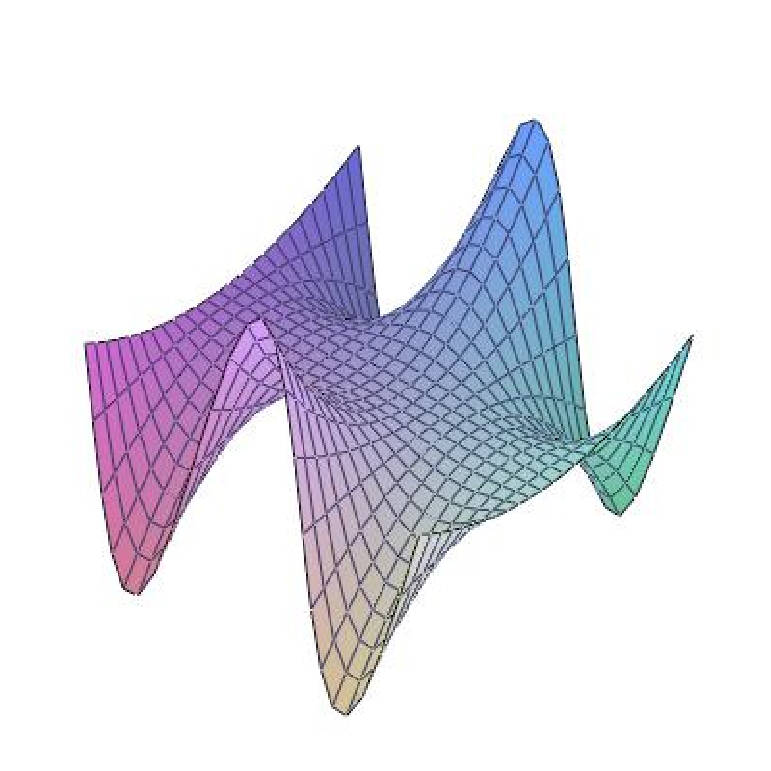
\includegraphics[scale=0.5]{grafica10.jpg}
\caption{Gráfica de $x^2 \cdot \cos (y)$}%Comando para ponerle nombre a la imagen
\end{figure}

\newpage

\section{Figuras y texto en línea}

%Se indica el entorno de figura en la página
\begin{figure}[h!]
	%Minipágina con cierto tamaño \begin{minipage}{tamaño de las columnas}
	\begin{minipage}{0.5\textwidth} %Se definen las columnas a utilizar en el entorno
		Ejemplo de uso de \emph{minipage} para colocar texto y figuras en línea.\\
		El texto se colocará a la izquierda de la página y la figura a la derecha.
	\end{minipage}
	\begin{minipage}{0.4\textwidth} %Ocupa el 40 de ancho de la caja de texto
		\centering
		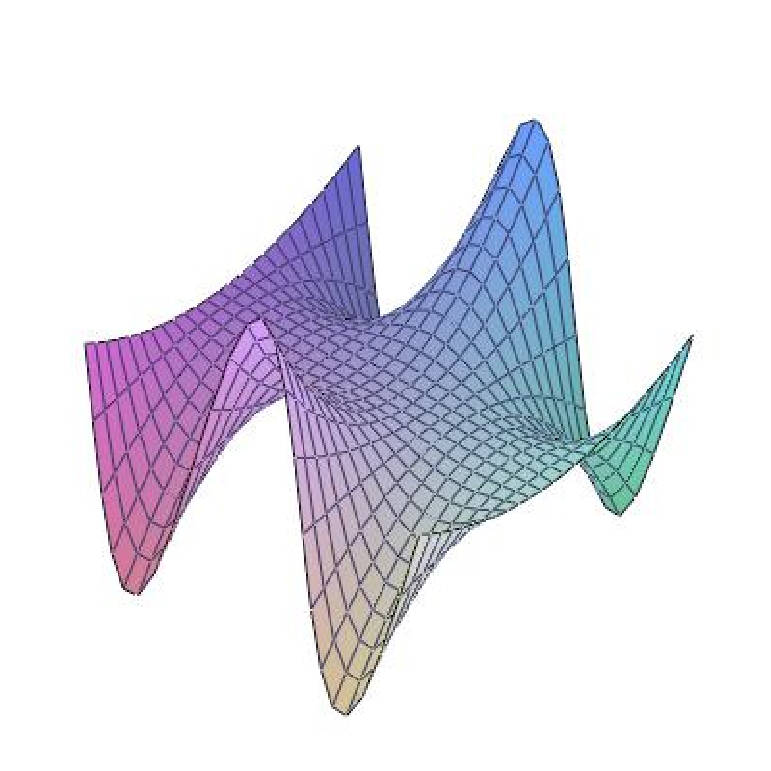
\includegraphics[scale=0.2]{grafica10.jpg}
		\caption{Gráfica 2}
	\end{minipage}
\end{figure}

\newpage

\section{Efectos}

\begin{figure}[h!]
\centering
% Scale => 1 agranda la imagen, si es scale<1 la reduce
% width=x-ancho, height=x-altura
%\includegraphics[opciones] opciones:angle,scale,height,width
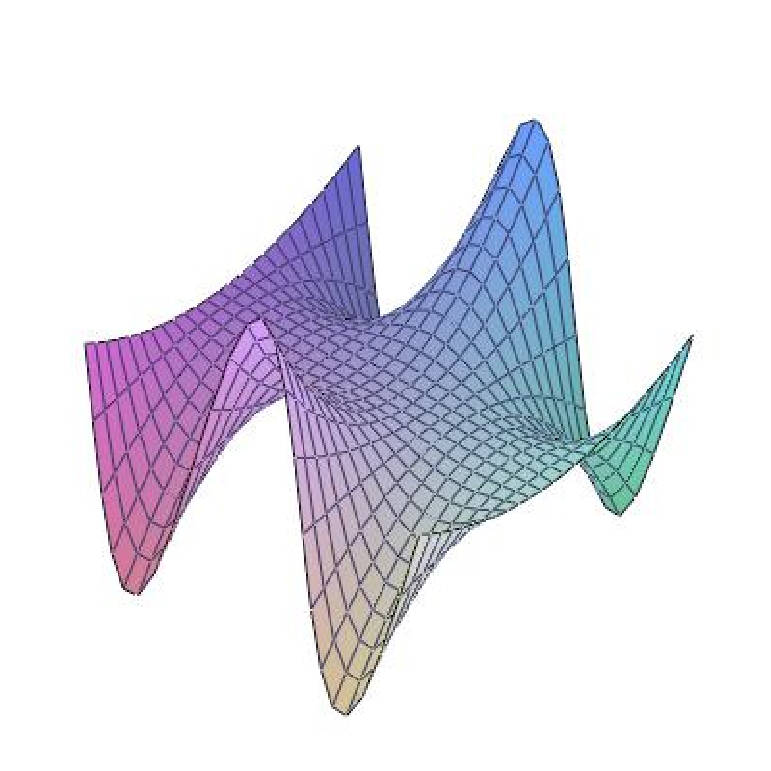
\includegraphics[angle=45,scale=0.5]{grafica10.jpg}
\caption{Gráfica de $x^2 \cdot \cos (y)$}
\end{figure}

\newpage

\section{Subfiguras}

\begin{figure}[h!]
	\centering	
	\subfigure[Ping\"uino]{
\includegraphics[angle=30,width=4cm]{pinguino}}
	\subfigure[Función]{\fbox{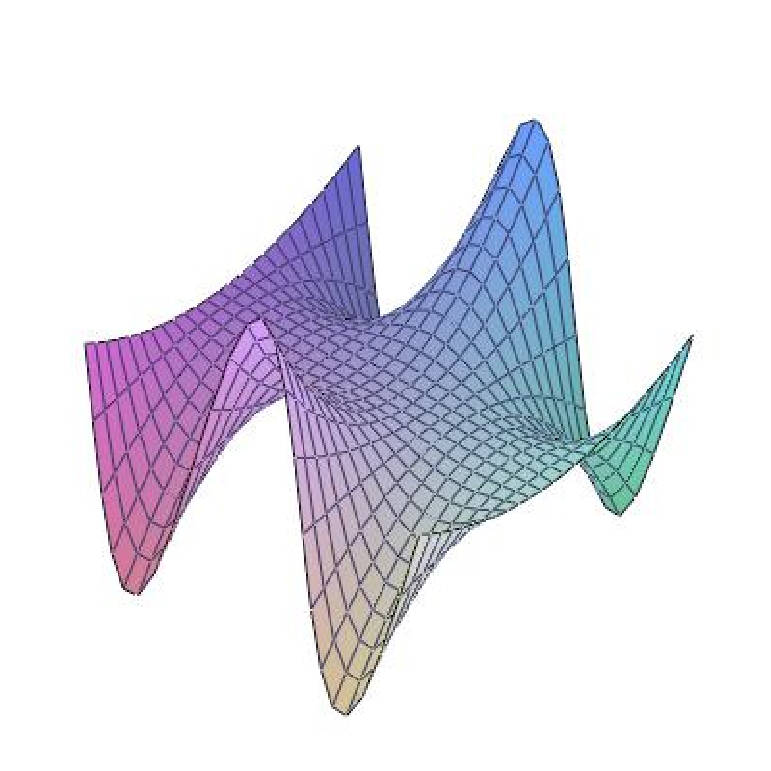
\includegraphics[width=4cm]{grafica10}}} %fbox coloca un marco a una imagen o texto
	\subfigure[Quijote]{
\includegraphics[width=3cm]{quijote}} %Se puede dar el tamaño de la figura como quiera
	\caption{Imagenes en línea}
\end{figure}

\begin{figure}[h!]
	\centering	
	\subfigure[Ping\"uino]{
\includegraphics[angle=30,width=4cm]{pinguino}}
	\subfigure[Función]{\fbox{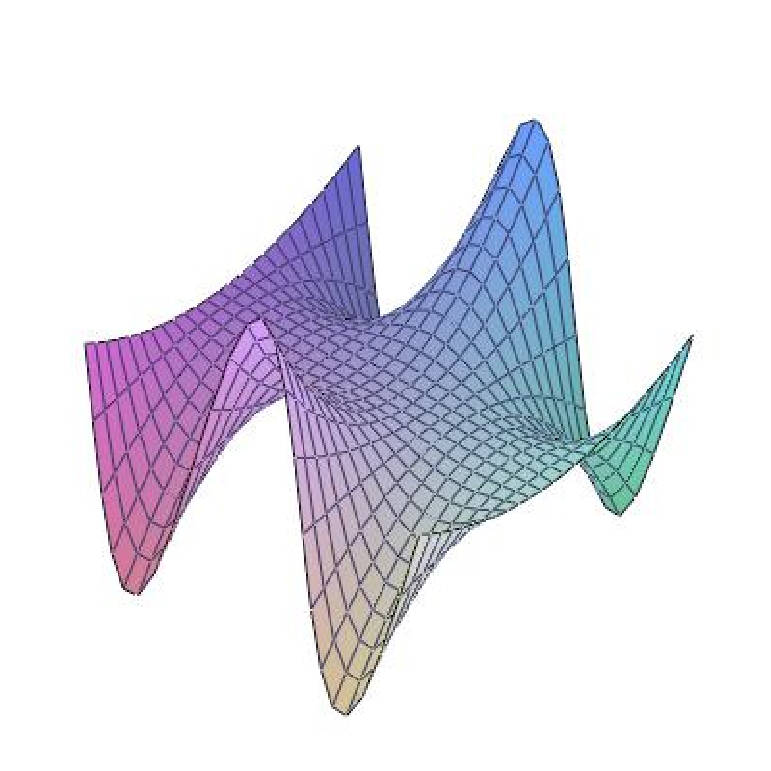
\includegraphics[width=4cm]{grafica10}}}
	\subfigure[Ping\"uino]{
\includegraphics[angle=30,width=4cm]{pinguino}}
	\subfigure[Función]{\fbox{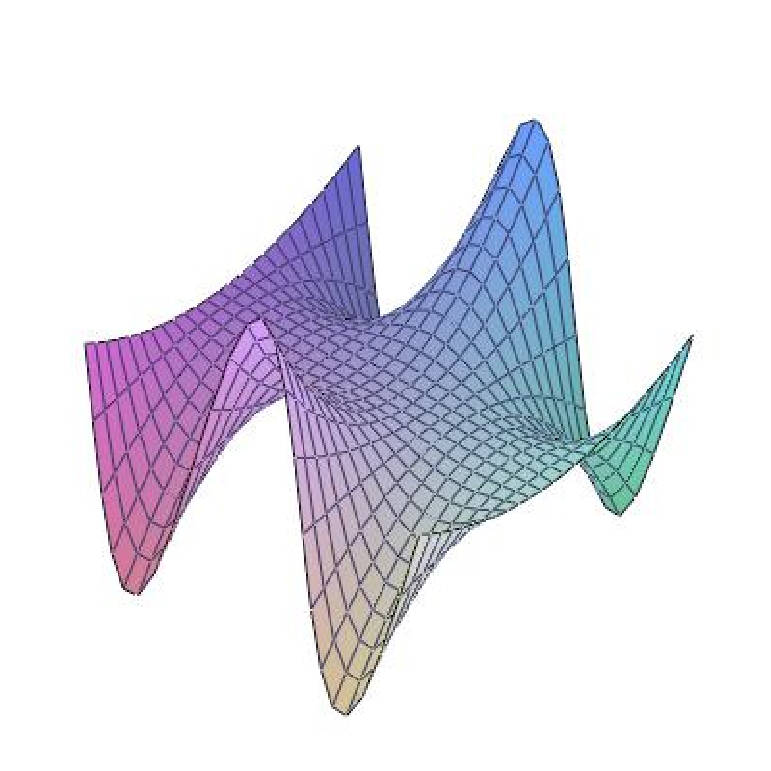
\includegraphics[width=4cm]{grafica10}}}
	\subfigure[Ping\"uino]{
\includegraphics[angle=30,width=4cm]{pinguino}}
	\subfigure[Función]{\fbox{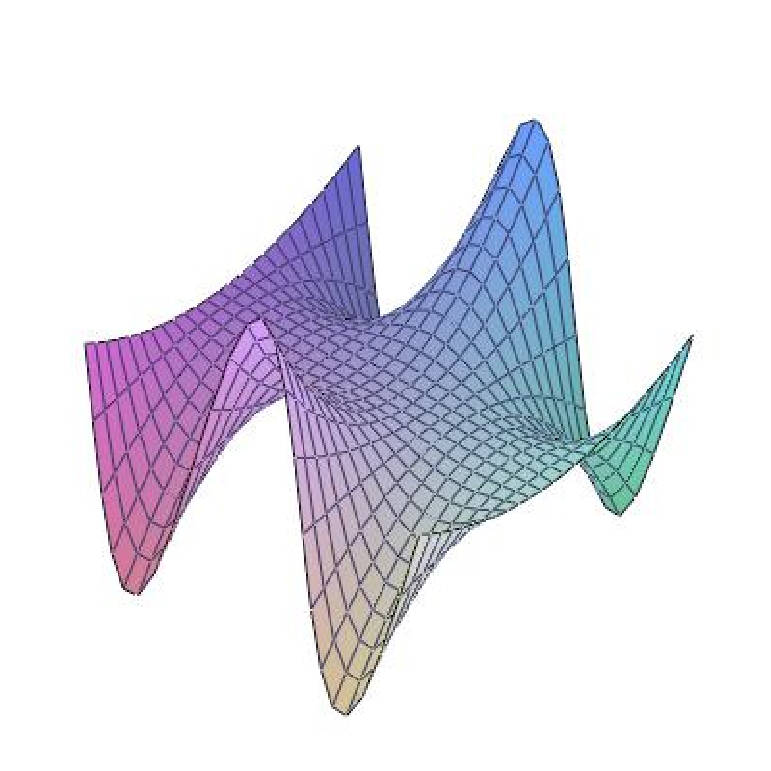
\includegraphics[width=4cm]{grafica10}}}
	\subfigure[Ping\"uino]{
\includegraphics[angle=30,width=4cm]{pinguino}}
	\subfigure[Función]{\fbox{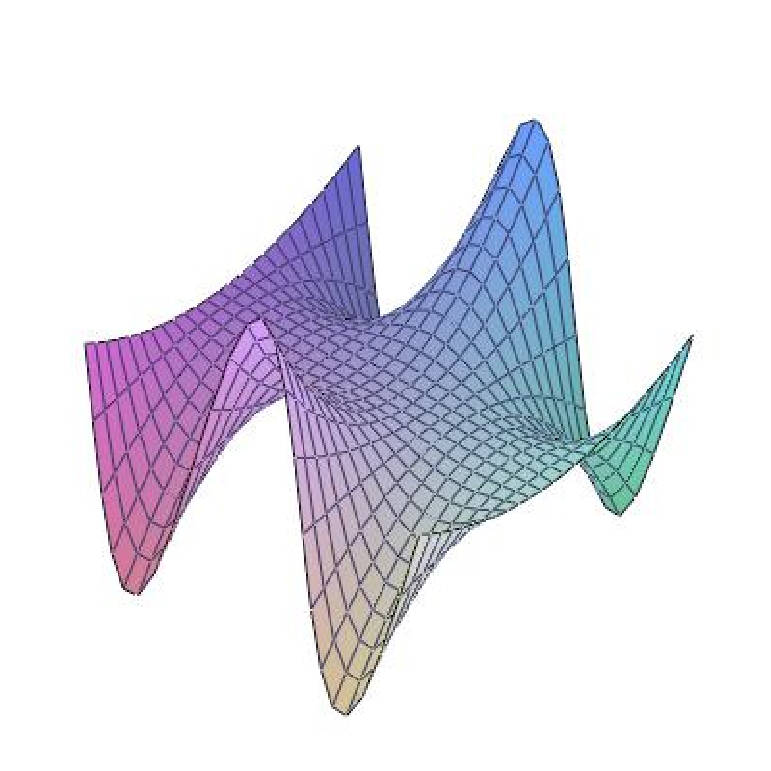
\includegraphics[width=4cm]{grafica10}}}
	\caption{Arreglo de imagenes}
\end{figure}
\newpage

\section{\fbox{Elementos} en línea con \textit{parbox}}
% framebox es otra manera de colocarle un marco a una imagen
\framebox{\parbox{5cm}{
\includegraphics[width=5cm]{quijote}}}
\addcontentsline{lof}{figure}{Quijote} %para agregar una figura que no esta en un caption
%\addcontentsline{donde se agrega la informacion}{tipo de entrada}{texto a agregar}
\hfill \parbox{11cm}{En un lugar de la Mancha, de cuyo nombre no quiero acordarme, 
no ha mucho tiempo que vivía un hidalgo de los de lanza en astillero, adarga antigua, 
rocín flaco y galgo corredor. Una olla de algo más vaca que carnero, salpicón las más 
noches, duelos y quebrantos los sábados, lentejas los viernes, algún palomino de añadidura 
los domingos, consumían las tres partes de su hacienda. El resto della concluían sayo 
de velarte, calzas de velludo para las fiestas con sus pantuflos de lo mismo, los días 
de entre semana se honraba con su vellori de lo más fino. Tenía en su casa una ama que 
pasaba de los cuarenta, y una sobrina que no llegaba a los veinte, y un mozo de campo 
y plaza, que así ensillaba el rocín como tomaba la podadera\dots }

\end{document}
